\section{Methods} 
\label{sec:rumiMethods}
Our objective here is to introduce information-theoretic metrics for evaluating classification performance in protein function prediction. In this learning scenario, the input space $\mathcal{X}$ represents proteins whereas the output space $\mathcal{Y}$ contains directed acyclic graphs describing protein function according to the Gene Ontology (GO). 

Because of the hierarchical nature of GO, both experimental and computational annotations need to satisfy the \emph{consistency requirements}:

\begin{enumerate}[label=\roman*.,font=\itshape]
\item

If vertex (term) $v$ from the ontology is true, then all of its ancestors must also be true.

\item
If vertex (term) $v$ from the ontology is false, then all of its descendants must also be false.

\end{enumerate}
By enforcing these requirements we frame the task of a classifier as assigning the best consistent subgraph of the ontology to each new protein and output a prediction score for this subgraph and/or each predicted term. 

We simplify the exposition by referring to such graphs as prediction or annotation graphs. In addition, we frequently treat consistent graphs as sets of nodes or functional terms and use set operations to manipulate them. %Finally, because we use Gene Ontology for describing protein function, we shall alternatively refer to the GO graph as an ontology. 

We now proceed to provide a definition for the information content of a (consistent) subgraph in the ontology. Then, using this definition, we derive information-theoretic performance evaluation metrics for comparing pairs of graphs.

%%%%%%%%%%%%%%%%%%%%%%
%%%%%%%%%%%%%%%%%%%%%%
\subsection{Calculating the joint probability of a graph}
%%%%%%%%%%%%%%%%%%%%%%
%%%%%%%%%%%%%%%%%%%%%%


Let each term in the ontology be a binary random variable and consider a fixed but unknown probability distribution over $\mathcal{X}$ and $\mathcal{Y}$ according to which the quality of a prediction process will be evaluated. We shall assume that the prior distribution of a target can be factorized according to the structure of the ontology, i.e. we assume a Bayesian network as the underlying data generating process for the target variable. According to this assumption, each term is independent of its ancestors given its parents and, thus, the full joint probability can be factorized as a product of individual terms obtained from the set of conditional probability tables associated with each term \citep{Koller2009}, 

\begin{equation}
\Pr(\mathbf{V})=\underset{v\in \mathbf{V} }{\prod}\Pr(v|\mathcal{P}(v)),
\label{eq:full_joint1}
\end{equation}
where $\mathbf{V}$ denotes all vertices the ontology, $v$ denotes a vertex in $\mathbf{V}$ and $\mathcal{P}(v)$ is the set of parent nodes of $v$.  Here we use $\mathbf{V}$ (all terms) instead of $T$ (only true terms) to illustrate the fact that we are calculating the probability of a given configuration of the full ontology with the inclusion of all true and false terms. In practice the true terms, or the subgraph $T$, are generally all that is considered both in the context of this chapter and in other papers addressing similar topics. 

%%%%%%%%%%%%%%%%%%%%%%
%%%%%%%%%%%%%%%%%%%%%%
\begin{figure}
\begin{centering}
\centering
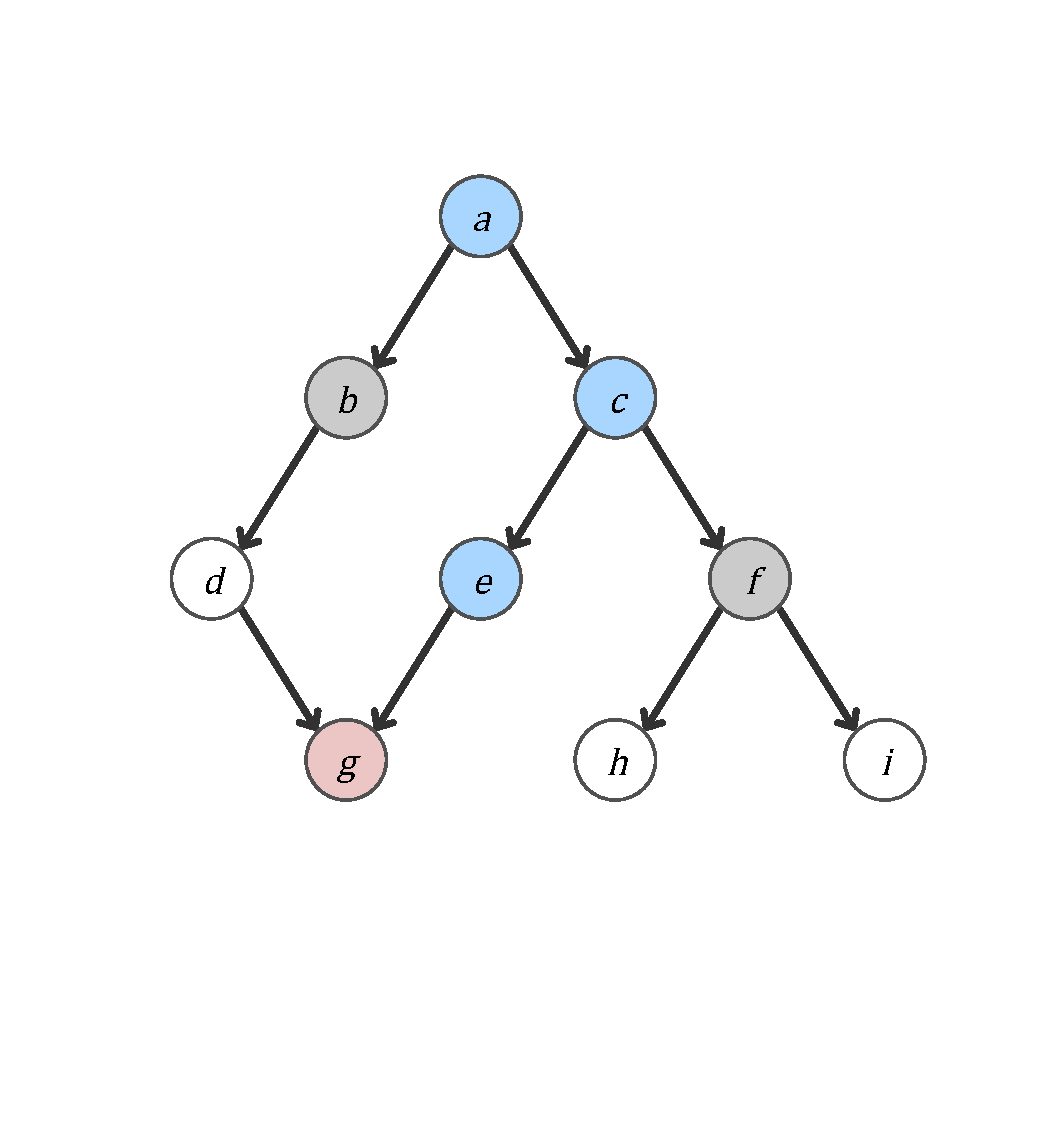
\includegraphics[scale=0.6]{Figures/rumi/full_joint_ontology}


\caption[A graph of terms illustrating different vertices used to calculate a full joint probability ]{ A directed acyclic graph representing the relationships between terms in an ontology. True term, or $T$, are represented by blue colored vertices: $\{ a, c, e\}$. The children of true terms, $\mathcal{C}(T)$, are denoted by grey and light-red vertices: $\{ b, f, g\}$. Terms which do not contribute anything to the full joint probability are shown in white and light-red: $\{d, g, h, i\}$. Term $g$ is colored light red to point out a special case when calculating the full joint probability of a graph.  Although one of term $g$'s parents are true, because it has one false parent it will not contribute to the calculation of the full joint probability because the probability it is false is always equal to one (\Cref{tab:rumiCPD}). All blue and grey terms taken together comprise the \emph{markov blanket} of $T$ and are necessary when calculating the full joint probability of a configuration, or combination of true and false values for all terms, in $\mathbf{V}$.}
\end{centering}
\label{fig:fulljoint}
\end{figure}

%%%%%%%%%%%%%%%%%%%%%%
%%%%%%%%%%%%%%%%%%%%%%

%Table
%%%%%%%%%%%%%%%%%%%%%%
%%%%%%%%%%%%%%%%%%%%%%

\begin{table*}[t]
\caption[A table of the joint probability distribution for variable $g$]{A table showing a conditional probability distribution for term $g$ from \Cref{fig:fulljoint}.  The purpose of this table is to illustrate how the consistency requirement affects joint probability tables in the bayesian network.   If at least one of a term's parents are false it is guaranteed that term is also false.  This is shown by considering the last three rows in the table.  
}

{\begin{tabular}{cc|cc}
\hphantom & \multicolumn{1}{c}{\hphantom} & \multicolumn{2}{c}{$\Pr(g)$}\\
$d$ & $e$ & True & False\\
\hline
True & True & .7 & .3\\
True & False & 0 & 1\\
False & True & 0 & 1\\
False & False & 0 & 1\\

\end{tabular}}
\label{tab:rumiCPD}
\end{table*}
%%%%%%%%%%%%%%%%%%%%%%
%%%%%%%%%%%%%%%%%%%%%%

The scope of terms considered can be reduced when calculating the joint probability of a configuration of $\mathbf{V}$ without affecting the final probability value. Because of the enforced consistency requirement (i.e. all ancestors of true terms are true; all descendants of false terms are false) the full joint probability of a configuration of the ontology, $\mathbf{V}$, can be calculated by considering only terms whose parents are all true. \Cref{eq:full_joint1} can be rewritten as

\begin{equation}
\Pr(\mathbf{V})=\underset{v\in T \cup \mathcal{C}(T)}{\prod}\Pr(v|\mathcal{P}(v)),
\label{eq:full_joint}
\end{equation}

\noindent where $T$ denotes all terms in $\mathbf{V}$ that are true, $\mathcal{C}(T)$ defines the children of all terms in $T$ (specifically, false terms all of whose parents are true), and  $T \cup \mathcal{C}(T)$ defines the unique union of the two sets. 

The derivation of \Cref{eq:full_joint} can be obtained by considering \Cref{fig:fulljoint} which illustrates a sample ontology with $9$ terms and \Cref{tab:rumiCPD} which represents the conditional probability distribution, or table, for vertex $g$.  If we write the joint probability of $\mathbf{V}$ using \Cref{eq:full_joint1} we obtain 
\begin{eqnarray*}
\Pr(\mathbf{V}) &= &\Pr(a=1) \times \Pr(b=0|a=1) \times \Pr(c=1|a=1) \times \Pr(d=0|b=0)\\
 & &  \times \Pr(e=1|c=1) \times \Pr(f=0|c=1) \times \Pr(g=0|d=0,e=1)\\
  & & \times \Pr(h=0|f=0) \times \Pr(i=0|f=0).
\end{eqnarray*}
First, we see that terms $h$ and $i$ contribute nothing to the joint probability because the probability a term is false given its parents are all false is always equal to 1.  Although $b$, and $f$ are false, because one of their parents are true the resulting probability is not 1.  Term $g$ can also be ignored because one of its parents is false.  For example, consider \Cref{tab:rumiCPD}, which shows the conditional probability table of term $g$.  If we consider instances where one of $g$'s parents are false we see that the resulting values are guaranteed to be 1. The resulting joint probability can subsequently be rewritten as 
\begin{eqnarray*}
\Pr (\mathbf{V}) & = &\Pr(a=1) \times \Pr(b=0|a=1) \times \Pr(c=1|a=1)\\  
 & & \times \Pr(e=1|c=1) \times \Pr(f=0|c=1).
\end{eqnarray*}

Because in practice most annotations only draw upon a small fraction of terms, most terms and their descendants, will be negative and will not contribute to the calculation of a given joint probability.  For this reason, although calculating the full joint probability has an asymptotic upper bound defined by the number of terms in the ontology, in practice it should have much lower complexity.

In this context, we are only interested in marginal probabilities that a protein is experimentally associated with a consistent subgraph $T$ in the ontology. This probability can be expressed as

\begin{equation}
\Pr(T)=\underset{v\in T}{\prod}\Pr(v|\mathcal{P}(v)).
\label{eq:factorization}
\end{equation}

\Cref{eq:factorization} can be derived from the full joint factorization by first marginalizing over the leaves of the ontology and then moving towards the root(s) for all nodes not in $T$.  

Although marginalizing over all negative terms gives a formulation that deviates from calculating the full joint probability it both simplifies calculating the information content of a sub-graph and can be philosophically justified. Unobserved annotations are only putative negative observations because explicit negative annotations are rarely deposited in biological databases.  In ignoring all negative terms we are implicitly recognizing that they are simply unobserved variables and not actual negative annotations.  

%%%%%%%%%%%%%%%%%%%%%%
%%%%%%%%%%%%%%%%%%%%%%
\subsection{Calculating the information content of a graph}
%%%%%%%%%%%%%%%%%%%%%%
%%%%%%%%%%%%%%%%%%%%%%

Now that we have properly defined the joint probability of a set of terms, or subgraph of the ontology, calculating the information content of those terms is relatively straightforward.  The information content of a subgraph can be thought of as the number of bits of information one would receive about a protein if it were annotated with that particular subgraph. We calculate the information content of a subgraph $T$ in a straightforward manner as

\[
i(T)=\log\frac{1}{\Pr(T)}
\]


\noindent and use a base 2 logarithm as a matter of convention. The information content of a subgraph $T$ can now be expressed by combining the previous two equations as

\begin{eqnarray*}
i(T) & = & \underset{v\in T}{\sum}\log\frac{1}{\Pr(v|\mathcal{P}(v))}\\
 & = & \underset{v\in T}{\sum}ia(v),
\end{eqnarray*}


\noindent where, to simplify the notation, we use $ia(v)$ to represent the negative logarithm of $\Pr(v|\mathcal{P}(v))$. Term $ia(v)$ can be thought of as the increase, or accretion, of information obtained by adding a child term to a parent term, or set of parent terms, in an annotation. We will refer to $ia(v)$ as \emph{information accretion} (perhaps information gain would be a better term, but because it is frequently used in other applications to describe an expected reduction in entropy, we avoid it in this situation).

A simple ontology containing five terms together with a conditional probability table associated with each node is shown in \Cref{fig:ontologytable}A. Note that because of the graph consistency requirement, each conditional probability table is limited to a single number. For example, at node $b$ in the graph, the probability $\Pr(b=1|a=1)$ is the only one necessary because $\Pr(b=0|a=1)=1-\Pr(b=1|a=1)$ and because $\Pr(b=1|a=0)$ is guaranteed to be $0$. In \Cref{fig:ontologytable}B we show a sample data set of four proteins functionally annotated according to the distribution defined by the Bayesian network. In \Cref{fig:ontologytable}C, we show the total information content for each of the four annotation graphs.

\begin{figure}
\noindent \begin{centering}
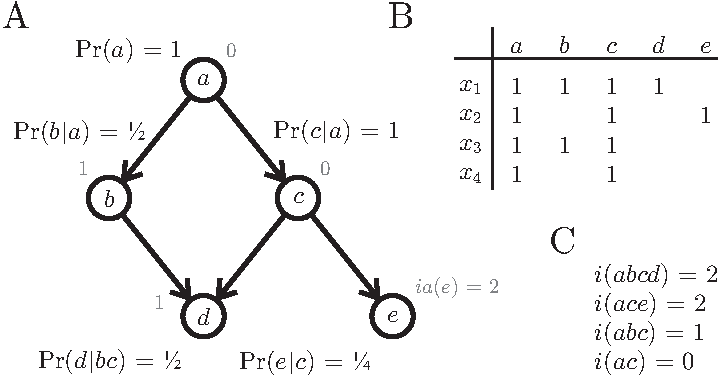
\includegraphics[scale=0.7]{Figures/rumi/ontology_table_v04}
\par\end{centering}

\caption[A sample ontology and data set illustrating calculating information content]{An example of an ontology, data set, and calculation of information content. (A) An ontology viewed as a Bayesian network together with a conditional probability table assigned to each node. Each conditional probability table is limited to a single number due to the consistency requirement in assignments of protein function. Information accretion calculated for each node, e.g. $ia(e)=-\log\Pr(e|c)=2$, are shown in grey next to each node. (B) A data set containing four proteins whose functional annotations are generated according to the probability distribution from the Bayesian network. (C) The total information content associated with each protein found in panel B; e.g. $i(ace)=ia(a)+ia(c)+ia(e)=2$. Note that $i(ab)=1$ and $i(abcde)=4$ although proteins with such annotation have not been observed in part B.}
\label{fig:ontologytable}
\end{figure}




%%%%%%%%%%%%%%%%%%%%%%
%%%%%%%%%%%%%%%%%%%%%%
\subsection{Comparing two annotation graphs}
%%%%%%%%%%%%%%%%%%%%%%
%%%%%%%%%%%%%%%%%%%%%%


We now consider a situation in which a protein's true and predicted function are represented by graphs $T$ and $P$, respectively. We define two metrics that can be thought of as the information-theoretic analogs of recall and precision, and refer to them as remaining uncertainty and misinformation, respectively. 

\textbf{Definition 1.} The \emph{remaining uncertainty} about the protein's true annotation corresponds to the information about the protein that is not yet provided by the graph $P$. More formally, we express the remaining uncertainty ($ru$) as

\begin{equation}
ru(T,P)=\underset{v\in T\setminus P}{\sum}ia(v),
\label{eq:ruSIMP}
\end{equation}


\noindent which is simply the total information content of the nodes in the ontology that are contained in true annotation $T$ but not in the predicted annotation $P$. Note that, in a slight abuse of notation, we apply set operations to graphs to manipulate only the vertices of these graphs. %which also indicates that the consistent graphs are treated here as sets of (weighted) nodes or functional terms. 

\textbf{Definition 2.} The \emph{misinformation} introduced by the classifier corresponds to the total information content of the nodes along incorrect paths in the prediction graph $P$. More formally, the misinformation is expressed as

\begin{equation}
mi(T,P)=\underset{v\in P\setminus T}{\sum}ia(v),
\label{eq:miSIMP}
\end{equation}


\noindent which quantifies how misleading a predicted annotation is. 

Here, a perfect prediction (one that achieves $P=T$) leads to $ru(T,P)=mi(T,P)=0$.  However, both $ru(T,P)$ and $mi(T,P)$ can be infinite in the limit. In practice, though, $ru(T,P)$ is bounded by the information content of the particular annotation, while $mi(T,P)$ is only limited by the number of annotations a predictor chooses to return. 


To illustrate calculation of remaining uncertainty and misinformation, in Figure 2 we show a sample ontology where the true annotation of a protein $T$ is determined by the two leaf terms $t_{1}$ and $t_{2}$, whereas the predicted subgraph $P$ is determined by the leaf terms $p_{1}$ and $p_{2}.$ The remaining uncertainty $ru(T,P)$ and misinformation $mi(T,P)$ can now be calculated by adding the information accretion corresponding to the nodes circled in grey. 

Finally, this framework can be used to define the similarity between the protein's true annotation and the predicted annotation without relying on identifying an individual common ancestor between pairs of leaves (this node is usually referred to as the maximum informative common ancestor; \citealt{Guzzi2012}). The information content of the subgraph shared by $T$ and $P$ is one such possibility; i.e. 
\[
s(T,P)=\underset{v\in T\cap P}{\sum}ia(v).
\]
%\textcolor{blue}{We define the similarity between the two sets as the information content of the common subgraph shared by them. More formally, we define this similarity as $s(T,P)=\underset{v\in T\cap P}{\sum}ia(v)$.}


%%%%%%%%%%%%%%%%%%%%%%
%%%%%%%%%%%%%%%%%%%%%%
\begin{figure}
\begin{centering}
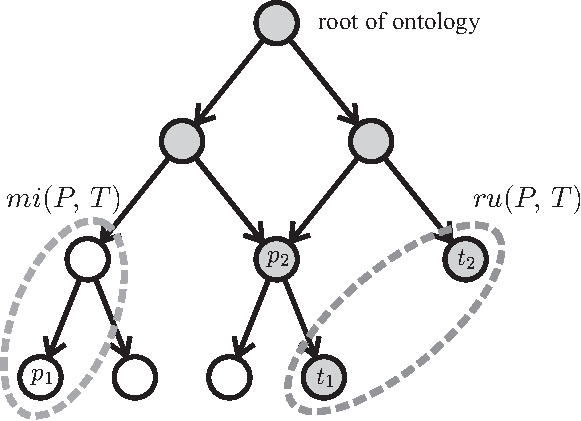
\includegraphics[scale=0.7]{Figures/rumi/ontology-rumi_v04}
\par\end{centering}

\caption[A graph showing terms used to calculate $ru$ and $mi$]{Illustration of calculating remaining uncertainty and misinformation given a predicted annotation graph $P$ and a graph of true annotations $T$. Graphs $P$ and $T$ are uniquely determined by the leaf nodes $p_{1}$, $p_{2}$, $t_{1}$, and $t_{2}$, respectively. Nodes colored in grey represent graph $T$. Nodes circled in grey are used to determine remaining uncertainty ($ru$; right side) and misinformation ($mi$; left side) between $T$ and $P$}.

\end{figure}
%%%%%%%%%%%%%%%%%%%%%%
%%%%%%%%%%%%%%%%%%%%%%


%%%%%%%%%%%%%%%%%%%%%%
%%%%%%%%%%%%%%%%%%%%%%
\subsection{Measuring the quality of function prediction}
%%%%%%%%%%%%%%%%%%%%%%
%%%%%%%%%%%%%%%%%%%%%%

A typical predictor of protein function usually outputs scores that indicate the strength (e.g. posterior probabilities) of predictions for each term in the ontology. To address this situation, the concepts of remaining uncertainty and misinformation need to be considered as a function of a decision threshold $\tau$. In such a scenario, predictions with scores greater than or equal to $\tau$ are considered positive predictions, while the remaining associations are considered negative (if the strength of a prediction is expressed via P-values or e-values, values lower than the threshold would indicate positive predictions). Regardless of the situation, every decision threshold results in a separate pair of values corresponding to the remaining uncertainty $ru(T,P(\tau))$ and misinformation $mi(T,P(\tau))$. 

The remaining uncertainty and misinformation for a previously unseen protein can be calculated as expectations over the data generating probability distribution. Practically, this can be performed by averaging over the entire set of proteins used in evaluation, i.e.

\begin{equation}
ru(\tau)=\frac{1}{n}\sum_{i=1}^{n}ru(T_{i},P_{i}(\tau))\label{eq:average_ru}
\end{equation}


\noindent and

\begin{equation}
mi(\tau)=\frac{1}{n}\sum_{i=1}^{n}mi(T_{i},P_{i}(\tau))\label{eq:average_mi}
\end{equation}


\noindent where $n$ is the number of proteins in the data set, $T_{i}$ is the true set of terms for protein $x_{i}$, and $P_{i}(\tau)$ is the set of predicted terms for protein $x_{i}$ given decision threshold $\tau$. Note that once the set of terms with scores greater than or equal to $\tau$ is determined, the set $P_{i}(\tau)$ is composed of the unique union of the ancestors of all predicted terms. As the decision threshold is moved from its minimum to its maximum value, the pairs of $(ru(\tau),mi(\tau))$ will result in a curve in 2D space. We refer to such a curve using $(ru(\tau),mi(\tau))_{\tau}$. Removing the normalizing constant ($\frac{1}{n}$) from the above equations would result in the total remaining uncertainty and misinformation associated with a database of proteins and a set of predictions.


%%%%%%%%%%%%%%%%%%%%%%
%%%%%%%%%%%%%%%%%%%%%%
\subsection{Weighted metrics}
%%%%%%%%%%%%%%%%%%%%%%
%%%%%%%%%%%%%%%%%%%%%%

One disadvantage of definitions in Equations \ref{eq:average_ru} and \ref{eq:average_mi} is that an equal weight is given to proteins with low and high information content annotations when averaging. To address this we assign a weight to each protein according to the information content of its experimental annotation. This formulation naturally downweights proteins with less informative annotations compared to proteins with rare, and therefore more informative (surprising), annotations. In biological data sets, frequently seen annotations have a tendency to be incomplete or shallow annotation graphs and arise due to the limitations or high-throughput nature of some experimental protocols. We define \emph{weighted remaining uncertainty} as

\begin{equation}
wru(\tau)=\frac{\sum_{i=1}^{n}i(T_{i})\cdot ru(T_{i},P_{i}(\tau))}{\sum_{i=1}^{n}i(T_{i})}
\label{eq:weighted_ru}
\end{equation}

\noindent and \emph{weighted misinformation} as

\begin{equation}
wmi(\tau)=\frac{\sum_{i=1}^{n}i(T_{i})\cdot mi(T_{i},P_{i}(\tau))}{\sum_{i=1}^{n}i(T_{i})}
\label{eq:weighted_mi}
\end{equation}


%\noindent \sout{A curve in the 2D space $(wru(\tau),wmi(\tau))_{\tau}$ can now be plotted and used to quantify or visualize the prediction quality for different classification models.}

%%%%%%%%%%%%%%%%%%%%%%
%%%%%%%%%%%%%%%%%%%%%%
\subsection{Semantic distance}
%%%%%%%%%%%%%%%%%%%%%%
%%%%%%%%%%%%%%%%%%%%%%

Finally, to provide a single performance measure which can be used to rank and evaluate protein function prediction algorithms, we introduce \emph{semantic distance} as the minimum distance from the origin to the curve $(ru(\tau),mi(\tau))_{\tau}$. More formally, the semantic distance $S_{k}$ is defined as

\begin{equation}
S_{k}=\underset{\tau}{\min}(ru^{k}(\tau)+mi^{k}(\tau))^{\frac{1}{k}},
\label{eq:semantic_distance}
\end{equation}

\noindent where $k$ is a real number $\ge 1$. Setting $k=2$ results in the minimum Euclidean distance from the origin. The preference for Euclidean distance ($k=2$) over say Manhattan distance ($k=1$) is to penalize unbalanced predictions with respect to the depth of predicted and experimental annotations. 

%\textcolor{blue}{One interesting property of $S_{k}$ is its relationship with the semantic measure proposed by \cite{Jiang1997}.  If one replaces $i(T)$ and $S(T,P)$ with our graph based definitions of information content and similarity, then we state, without proof, that $S_{k}$ is equivalent to Jiang and Conrath's metric when $k=1$.}

%%%%%%%%%%%%%%%%%%%%%%
%%%%%%%%%%%%%%%%%%%%%%
\subsection{Precision and recall}
%%%%%%%%%%%%%%%%%%%%%%
%%%%%%%%%%%%%%%%%%%%%%

In order to contrast the semantic distance-based evaluation with more conventional performance measures, in this section we briefly introduce precision and recall for measuring functional similarity. As before, we consider a set of propagated experimental terms $T$ and predicted terms $P(\tau)$, and define precision as the fraction of terms predicted correctly. More specifically, 

\[
pr(T,P(\tau))=\frac{|T\cap P(\tau)|}{|P(\tau)|},
\]

\noindent where $\left|\cdot\right|$ is the set cardinality operator.  Only proteins for which the prediction set is non-empty can be used to calculate average precision.  To address this issue the root term is counted as a prediction for all proteins. Similarly, recall is defined as the fraction of experimental (true) terms which were correctly predicted, i.e.

\[
rc(T,P(\tau))=\frac{|T\cap P(\tau)|}{|T|}.
\]


\noindent As before, precision $pr(\tau)$ and recall $rc(\tau)$ for the entire data set are calculated as averages over the entire set of proteins (note that an alternative definition of precision and recall given by \citealt{Verspoor2006} is described in \Cref{sec:rumiAddTop}). Finally, to provide a single evaluation measure we use the maximum F-measure over all decision thresholds. For a particular set of terms $T$ and $P(\tau)$, F-measure is calculated as the harmonic mean of precision and recall. More formally, the final evaluation metric is calculated as

\begin{equation}
F_{\max}=\underset{\tau}{\max}\left\{ 2\cdot\frac{pr(\tau)\cdot rc(\tau)}{pr(\tau)+rc(\tau)}\right\} 
\label{eq:fmax}
\end{equation}


\noindent where $pr(\tau)$ and $rc(\tau)$ are calculated by averaging over the data set. 

%%%%%%%%%%%%%%%%%%%%%%
%%%%%%%%%%%%%%%%%%%%%%
\subsubsection{Information-theoretic weighted formulation}
%%%%%%%%%%%%%%%%%%%%%%
%%%%%%%%%%%%%%%%%%%%%%

The definition of information accretion and the use of a probabilistic framework defined by the Bayesian network enables the straightforward application of information accretion to weight each term in the ontology. Therefore, it is easy to generalize the definitions of precision and recall from the previous section into a weighted formulation. Here, weighted precision and weighted recall can be expressed as

\[
wpr(T,P(\tau))=\frac{\underset{v\in T\cap P(\tau)}{\sum}ia(v)}{\underset{v\in P(\tau)}{\sum}ia(v)}
\]


\noindent and

\[
wrc(T,P(\tau))=\frac{\underset{v\in T\cap P(\tau)}{\sum}ia(v)}{\underset{v\in T}{\sum}ia(v)}.
\]


\noindent  Weighted precision $wpr(\tau)$ and recall $wrc(\tau)$ can then be calculated as weighted averages over the database of proteins, as in Equations \ref{eq:weighted_ru} and \ref{eq:weighted_mi}.

In addition to weighted precision and recall our framework also facilitates calculating weighted specificity

\[
%wsp(T,P(\tau))=\frac{ \underset{v\in \stcomp{T} \cap \stcomp{P} }{\sum}ia(v)}{\underset{v\in \stcomp{T}}{\sum}ia(v)}
wsp(T,P(\tau))=\frac{\underset{v\in T^{\bf{c}} \cap P^{\bf{c}}(\tau)}{\sum}ia(v)}{\underset{v\in T^{\bf{c}}}{\sum}ia(v)}
\]
where $T^{\bf{c}}$ represents the complement of set $T$ ($G \setminus T$).

%%%%%%%%%%%%%%%%%%%%%%
%%%%%%%%%%%%%%%%%%%%%%
\subsection{Supplementary evaluation metrics}
\label{sec:rumisupmethods}
%%%%%%%%%%%%%%%%%%%%%%
%%%%%%%%%%%%%%%%%%%%%%

When calculating remaining uncertainty, misinformation, precision and recall only consistent subgraphs of the Gene Ontology were considered. Under this framework, if a protein is annotated with multiple terms (either experimentally determined or predicted), as in \Cref{fig:ontologytable} , we determine consistent graphs $T$ (true) or $P$ (predicted) by recursively propagating annotations towards the root(s) of the ontology and taking a union of all terms encountered along the way. In each of these measures, it is sufficient to only consider vertices (terms) in the annotation graphs and calculate the similarity measure by manipulating vertices in an additive fashion. For example, each vertex in $T$ or $P$ counts equally in the precision/recall-based evaluation while the information accretion is used to weight the vertices in the ru-mi-based evaluation. 

A distinctly different approach can be taken by considering, on an individual basis, each leaf term that comprises a set $T$ or $P$. This is the approach taken to calculate various information-theoretic metrics \citep{Resnik1995, Jiang1997, Lin1998, Lord2003, Schlicker2006} as well as to provide an alternative definition of precision and recall \citep{Verspoor2006}. In this context the sets of leaf terms that define $T$ and $P$ (which we refer to as $\mathcal{L}(T)$ and $\mathcal{L}(P)$ respectively, and formally introduce below) are used to calculate a given metric. After calculating all pairwise metrics between the leaf terms, several different methods for averaging these scores can be applied to create a single similarity (or distance) value between $T$ and $P$.  We discuss these approaches below.

%%%%%%%%%%%%%%%%%%%%%%
%%%%%%%%%%%%%%%%%%%%%%
\subsubsection{Basic definitions}
%%%%%%%%%%%%%%%%%%%%%%
%%%%%%%%%%%%%%%%%%%%%%

Suppose we are given an ontology in the form of directed acyclic graph $G=(V, E)$, where $V$ is a set of vertices and $E\subset V\times V$ is the set of edges. In this graph, given an edge $(u,v) \in E$, we refer to vertex $u$ as a parent of $v$ and, alternatively, to vertex $v$ as a child of $u$. We also consider a set of all ancestors of $v$, $\mathcal{A}(v)$, and find this set by recursively identifying parents of all discovered nodes starting with $v$ until the root(s) of the ontology is (are) reached. For mathematical convenience, we consider vertex $v$ to be a member of $\mathcal{A}(v)$. Finally, given two vertices $u$ and $v$, we define a set of common ancestor nodes between these two vertices as $\mathcal{A}(u,v)$. Thus, $\mathcal{A}(u,v)= \mathcal{A}(u)\cap \mathcal{A}(v)$.

Consider now a consistent annotation graph $T$, where the set of vertices in $T$ is a subset of vertices in $G$. We define $\mathcal{L}(T)$, or the set of leaf terms represented by $T$, as

\begin{equation}
\mathcal{L}(T)=\{u : u \in T \land \lnot\exists ( (u, v) \in E  \land v \in T)\}.
\end{equation}

\noindent
In other words, $\mathcal{L}(T)$ contains only those vertices (terms) from $T$ that do not have children in $T$. Thus, the leaf terms are defined with respect to a particular annotation graph $T$ and generally differ from the leaf nodes in the ontology. 

%%%%%%%%%%%%%%%%%%%%%%
%%%%%%%%%%%%%%%%%%%%%%
\subsubsection{Information-theoretic metrics between pairs of vertices}
%%%%%%%%%%%%%%%%%%%%%%
%%%%%%%%%%%%%%%%%%%%%%

When calculating the information\hyp{}theoretic metrics of \citet{Resnik1995}, \citet{Jiang1997}, \citet{Lin1998}, \citet{Lord2003}, and \citet{Schlicker2006}, we calculate the information content of an individual term $v \in V$ as

\begin{equation}
i(v)=\log\frac{1}{\Pr(v)}
\end{equation}

\noindent
where $\Pr(v)$ can be calculated as the relative frequency of term $v$ among experimentally annotated proteins. The similarity between two distinct terms $u$ and $v$ as defined by \citet{Resnik1995} was calculated as

\begin{equation}
s_{R}(u,v)=\underset{w\in \mathcal{A}(u,v)}{\max}\{i(w)\},
\end{equation}

\noindent where $\mathcal{A}(u, v)$, as mentioned above, defines the set of common ancestors of terms $u$ and $v$. Similarity as defined by \citet{Lin1998} was calculated as

\begin{equation}
s(u,v)=\frac{s_{R}(u,v)}{i(u)+i(v)},
\end{equation}

\noindent and as defined by \citet{Schlicker2006} as

\begin{equation}
s(u,v)=\frac{s_{R}(u,v)}{i(u)+i(v)}\cdot(1-\underset{w\in \mathcal{A}(u,v)}{\min}\{\Pr(w)\}).
\end{equation}

\noindent Finally, the distance metric defined by \citet{Jiang1997} was calculated as

\begin{equation}
d(u,v)=i(u)+i(v)-2 \cdot s_{R}(u,v).
\end{equation}

%%%%%%%%%%%%%%%%%%%%%%
%%%%%%%%%%%%%%%%%%%%%%
\subsubsection{Information-theoretic metrics between pairs of graphs}
\label{sec:averaging}
%%%%%%%%%%%%%%%%%%%%%%
%%%%%%%%%%%%%%%%%%%%%%


Since the above metrics are only defined for two distinct terms, it is necessary to provide a mechanism to utilize these metrics in instances where a protein is annotated with graphs containing multiple leaf terms. Given two non-empty consistent annotation graphs of true and predicted terms, $T$ and $P$, and the set of leaf terms that define each set, $\mathcal{L}(T)$ and $\mathcal{L}(P)$, we employed two strategies for averaging. In the first case values were averaged between all possible pairs of terms in $\mathcal{L}(T)$ and $\mathcal{L}(P)$. Specifically, we calculated $s(T,P)$ as 

\begin{equation}
s(T, P)=\frac{1}{|\mathcal{L}(T)|\cdot|\mathcal{L}(P)|}\underset{t\in\mathcal{L}(T)}{\sum}\underset{p\in\mathcal{L}(P)}{\sum}s(t,p).
\end{equation}

\noindent We refer to this form of averaging as \emph{all-pair} averaging. This method of averaging was applied by \citet{Lord2003} in calculating similarity between two functional annotations.

In the second case we calculated the similarity between the two sets as the average of the maximum similarity between a term from one set and all terms in the other.  Specifically, we calculated $s(T,P)$ as 

\begin{equation}
s(T, P)=\frac{1}{2|\mathcal{L}(T)|}\underset{t\in\mathcal{L}(T)}{\sum}\underset{p\in\mathcal{L}(P)}{\max}\{s(t,p)\}+\frac{1}{2|\mathcal{L}(P)|}\underset{p\in\mathcal{L}(P)}{\sum}\underset{t\in\mathcal{L}(T)}{\max}\{s(t, p)\}.
\label{eq:maxaverage}
\end{equation}

\noindent This measure represents the technique of averaging employed by \citet{Verspoor2006} when calculating precision and recall (originally referred to as hierarchical precision and recall). There, the authors separately calculate precision as

\begin{equation}
pr(T, P)=\frac{1}{|\mathcal{L}(P)|}\underset{p\in\mathcal{L}(P)}{\sum}\underset{t\in\mathcal{L}(T)}{\max}\frac{|\mathcal{A}(t,p)|}{|\mathcal{A}(p)|}
\end{equation}

\noindent and recall as

\begin{equation}
rc(T, P)=\frac{1}{|\mathcal{L}(T)|}\underset{t\in\mathcal{L}(T)}{\sum}\underset{p\in\mathcal{L}(P)}{\max}\frac{|\mathcal{A}(t,p)|}{|\mathcal{A}(t)|}.
\end{equation}

\noindent We refer to this method of averaging as \emph{max-average}. Although not implemented here, \citet{Schlicker2006} employ a technique for averaging that is similar to \Cref{eq:maxaverage}, but takes the maximum average similarity for one set as opposed to the average between the two. Specifically,

\begin{equation}
s(T, P)=\max \left\{ \frac{1}{|\mathcal{L}(T)|}\underset{t\in\mathcal{L}(T)}{\sum}\underset{p\in\mathcal{L}(P)}{\max}\{s(t,p)\},\frac{1}{|\mathcal{L}(P)|}\underset{p\in\mathcal{L}(P)}{\sum}\underset{t\in\mathcal{L}(T)}{\max}\{s(t,p)\} \right\} 
\end{equation}

\noindent When averaging pairwise comparisons for distance metrics, the above averages are calculated as the average of minimum pairwise distances instead of maximum pairwise similarities.  

%%%%%%%%%%%%%%%%%%%%%%
%%%%%%%%%%%%%%%%%%%%%%
\subsection{Additional topological metrics}
\label{sec:rumiAddTop}
%%%%%%%%%%%%%%%%%%%%%%
%%%%%%%%%%%%%%%%%%%%%%

In addition to information-theoretic metrics, we also used Jaccard's similarity coefficient \citep{jaccard1901} when calculating the similarity between the two consistent annotation graphs $T$ and $P$. The Jaccard similarity coefficient is defined as

\begin{equation}
s(T,P)=\frac{|T\cap P|}{|T\cup P|}.
\end{equation}

\noindent We note that cosine similarity as well as Maryland bridge coefficient \citep{Glazko2005} usually result in values correlated with the Jaccard similarity coefficient. For that reason, these two similarity measures were not presented.

